\subsection{Docking}
\begin{frame}{Molecular Docking}
\begin{columns}
\column{0.5\textwidth}
\begin{itemize}
	\item Estimates binding affinity between a ligand and protein
	\item Samples translational, rotational and conformations space of the ligand
	\item Uses a numerical scoring function	
	\item Highly parameterised meaning accuracy is system dependant
\end{itemize}
\column{0.5\textwidth}
\begin{figure}
\includegraphics[width=0.95\textwidth]{figures/theory/docking.png}
\end{figure}
\end{columns}
\end{frame}

\begin{frame}{gnina}
\begin{figure}
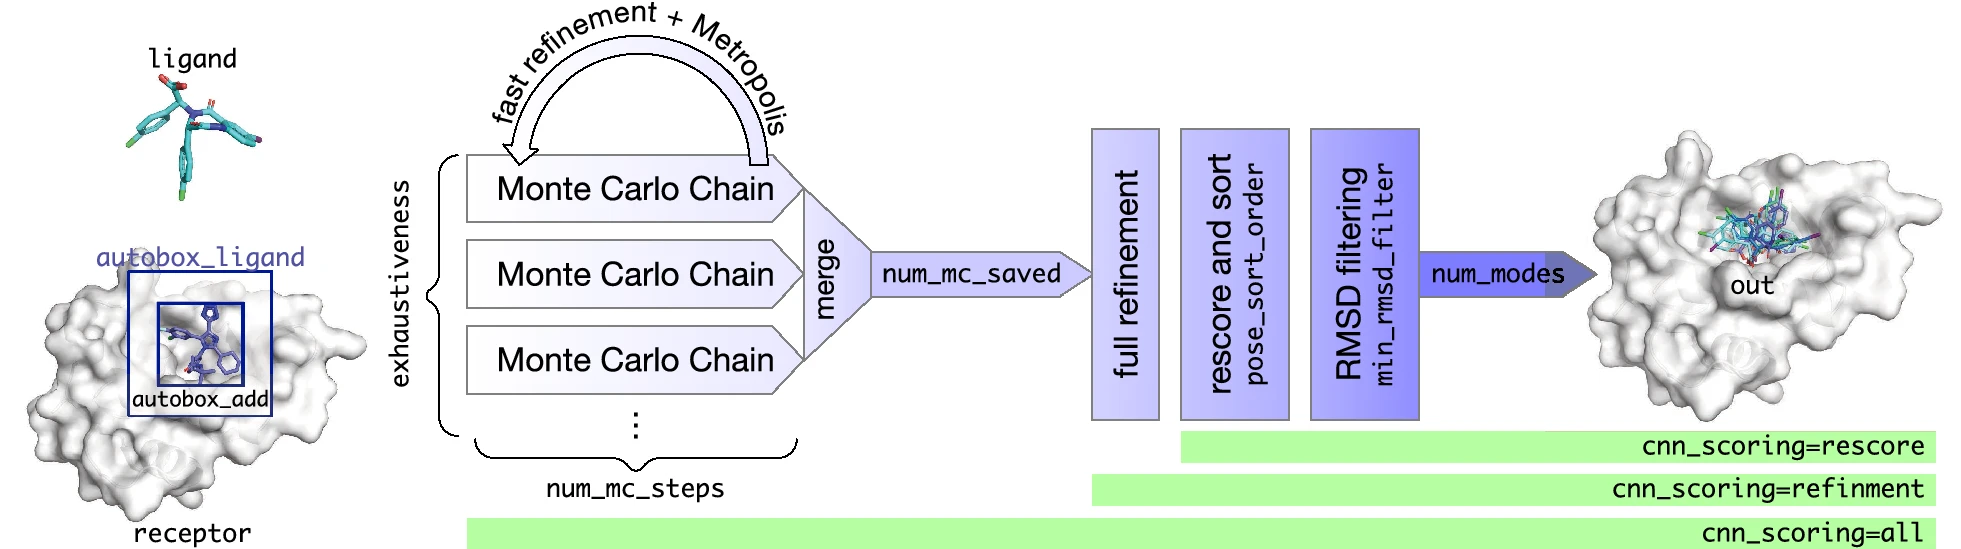
\includegraphics[height=0.4\textheight]{figures/theory/gnina.png}
\end{figure}
\begin{itemize}
	\item Uses Monte Carlo methods to sample conformational space
	\item Initially scores using an empirical scoring function
	\item Uses Convoluted Nural Networks to re-score and improve performance
\end{itemize}
{\tiny
McNutt, A.T., Francoeur, P., Aggarwal, R. et al. GNINA 1.0: molecular docking with deep learning. J Cheminform \textbf{13}, 43 (2021)}
\end{frame}